\subsection{直线和平面的位置关系}\label{subsec:1-7}

我们观察教室的墙面和地面,它们的相交线在地面上;
两墙面的相交线和地面只相交于一点;墙面和天花板的相交线和地面没有交点。
它反映出直线和平面之间存在着不同的位置关系。

如果一条直线和一个平面没有公共点,那么我们说\zhongdian{这条直线和这个平面平行}。

一条直线和一个平面的位置关系有且只有以下三种:

(1)\zhongdian{直线在平面内} —— 有无数个公共点;

(2)\zhongdian{直线和平面相交} —— 有且只有一个公共点;

(3)\zhongdian{直线和平面平行} —— 没有公共点。

我们把直线和平面相交或平行的情况统称为\zhongdian{直线在平面外}。

图 \ref{fig:ltjh-1-19} 是表示这三种位置关系的图形。一般地,
直线 $a$ 在平面 $\alpha$ 内时,应把直线 $a$ 画在表示平面 $\alpha$ 的平行四边形内;
直线 $a$ 在平面 $\alpha$ 外时,表示直线的线段要有一部分或全部画在表示平面 $\alpha$ 的平行四边形外。

\begin{figure}[htbp]
    \centering
    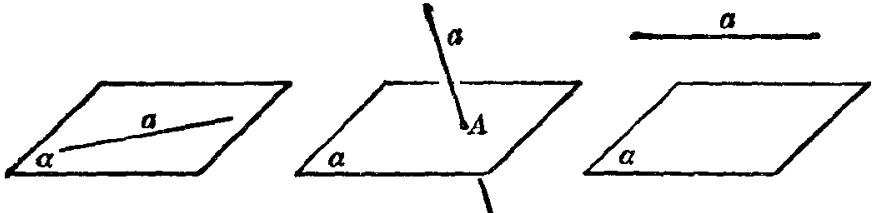
\includegraphics[width=11cm]{../pic/ltjh-ch1-19.png}
    \caption{}\label{fig:ltjh-1-19}
\end{figure}

直线 $a$ 与平面 $\alpha$ 相交于点 $A$,规定记作 $a \cap \alpha = A$;
直线 $a$ 与平面 $\alpha$ 平行,记作 $a \pingxing \alpha$;
直线 $a$ 在平面 $\alpha$ 外,记作 $a \not \subset \alpha$。


\begin{lianxi}

\xiaoti{观察图中的吊桥。说出立柱和桥面、水面,铁轨和桥面、水面的位置关系。}

\begin{figure}[htbp]
    \centering
    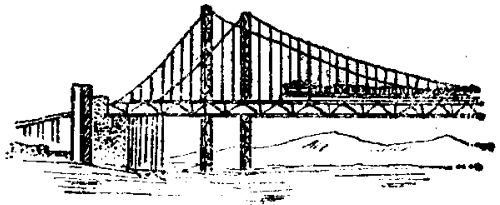
\includegraphics[width=7cm]{../pic/ltjh-ch1-subsec7-lx-01.png}
    \caption*{(第 1 题)}
\end{figure}


\xiaoti{举出直线和平面三种位置关系的实例。}

\end{lianxi}

